\section{Introduction}

In this master's thesis we will present a method to find timebounds for arbitrary integer programs.
\todo{Provide information about existing tools CoFloCo, KoAT, Loopus, ...}{There exist complexity analysis tools which already address the same task.}

The method of this master's thesis is based on the work of KoAT \cite{koat}.
It changes the methods of KoAT, such that the restriction for non-monotonic bounds is no longer necessary.
As a result the method is now able to infer non-monotonic time bounds.

We now take a look at an example to see the benefit of non-monotonic bounds.
Figure \ref{fig:motivational_example} shows a program, which takes two variables $x$ and $y$ as input and runs a loop, which decrements $x$ in each step with $t_1$ until $x$ is not greater than 0 anymore.
We can easily see, that the transition $t_1$ will be used at most $\max \braced{0, x-y}$ times.
However, since the previous method only used monotonic bounds, it only infers the bound $\abs{x}+\abs{y}$ for $t_1$.

\todo{Take a look at why lower time bounds are not an option}{}

\subsection{Motivation}

\begin{figure}
  \centering
  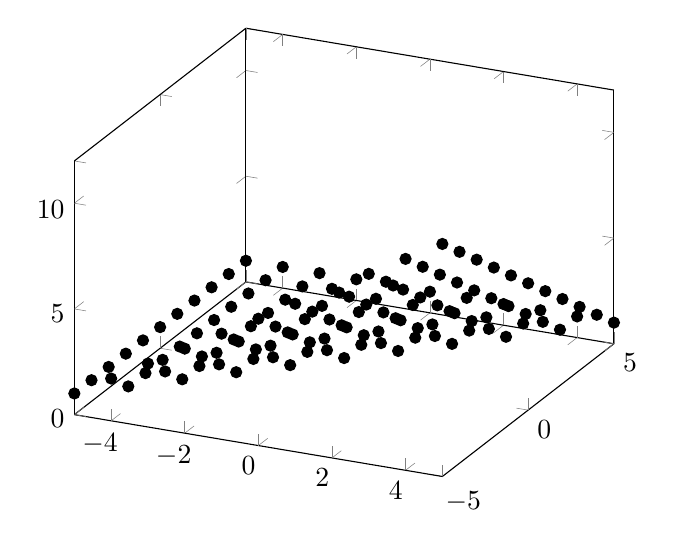
\begin{tikzpicture}
    \begin{axis}
      \addplot3 [
        unbounded coords=jump,
        mesh,
        shader=interp,
        samples at={-5,...,5},
        samples y={11},
        only marks,
      ] {1+max(x-y,0)};
    \end{axis}
  \end{tikzpicture}
  \hfil
  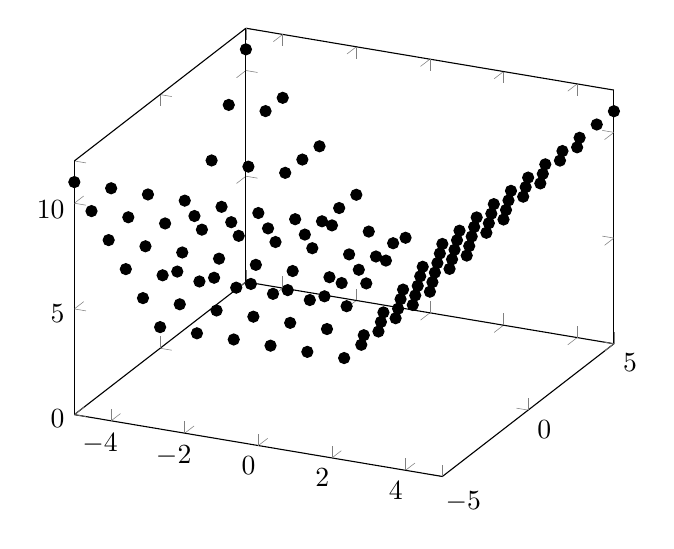
\begin{tikzpicture}
    \begin{axis}
      \addplot3 [
        unbounded coords=jump,
        mesh,
        shader=interp,
        samples at={-5,...,5},
        samples y={11},
        only marks,
      ] {1+abs(max(x,-y))+abs(max(x,-y))};
    \end{axis}
  \end{tikzpicture}
  \caption{Evaluation of the motivational example}
  \label{fig:motivational_evaluation}
\end{figure}


\begin{figure}
\centering
\begin{tikzpicture}[->,>=stealth',auto,node distance=5cm,
    thick,
    main node/.style={circle,draw,font=\sffamily\Large\bfseries},
    aligned edge/.style={align=left}]

  \node[main node] (0) {$l_0$};
  \node[main node] (1) [right of=0] {$l_1$};

  \path[every node/.style={font=\sffamily\small}]
    (0) edge[aligned edge] node {$t_0: x' = x \wedge y' = y$} (1)
    (1) edge[aligned edge, loop right] node {$t_1: x > 0 \wedge x' = x - 1 \wedge y' = -2 \cdot y$} (1)
    ;
\end{tikzpicture}
\caption{Program, where non-monotonic bounds does not yield a benefit}
\label{fig:non_beneficial_example}
\end{figure}

